% --------------------------------------------------------------
% This is all preamble stuff that you don't have to worry about.
% Head down to where it says "Start here"
% --------------------------------------------------------------
 
\documentclass[12pt]{article}
 
\usepackage[margin=1in]{geometry} 
\usepackage{amsmath,amsthm,amssymb, graphicx}
 \usepackage{algorithm}
\usepackage{algorithmic}

\newcommand{\N}{\mathbb{N}}
\newcommand{\Z}{\mathbb{Z}}
 
\newenvironment{theorem}[2][Theorem]{\begin{trivlist}
\item[\hskip \labelsep {\bfseries #1}\hskip \labelsep {\bfseries #2.}]}{\end{trivlist}}
\newenvironment{lemma}[2][Lemma]{\begin{trivlist}
\item[\hskip \labelsep {\bfseries #1}\hskip \labelsep {\bfseries #2.}]}{\end{trivlist}}
\newenvironment{exercise}[2][Exercise]{\begin{trivlist}
\item[\hskip \labelsep {\bfseries #1}\hskip \labelsep {\bfseries #2.}]}{\end{trivlist}}
\newenvironment{problem}[2][Problem]{\begin{trivlist}
\item[\hskip \labelsep {\bfseries #1}\hskip \labelsep {\bfseries #2.}]}{\end{trivlist}}
\newenvironment{question}[2][Question]{\begin{trivlist}
\item[\hskip \labelsep {\bfseries #1}\hskip \labelsep {\bfseries #2.}]}{\end{trivlist}}
\newenvironment{corollary}[2][Corollary]{\begin{trivlist}
\item[\hskip \labelsep {\bfseries #1}\hskip \labelsep {\bfseries #2.}]}{\end{trivlist}}

\newenvironment{solution}{\begin{proof}[Solution]}{\end{proof}}
 
\begin{document}
 
% --------------------------------------------------------------
%                         Start here
% --------------------------------------------------------------
 
 
% Your write-up should contain:
% the names of the people in your group (and each member's contribution),
% the optimizations used or attempted,
% the results of those optimizations,
% the reason for any odd behavior (e.g., dips) in performance, and
% how the performance changed when running your optimized code on a different machine. 
\title{CS 267 Homework 1 Part 2}
\author{Xingyou Song \footnote{xsong@berkeley.edu - Xingyou wrote the report, presented techniques and strategies for optimization, and coded some parts}, Yao Yuan \footnote{yao\_yuan@berkeley.edu - Yao coded a significant part of the code in C and tested using various compiler settings} \footnote{Our Third Partner, Zhiwei Yao, dropped the course.}} %replace with your name
\date{Due Feburary 9, 2018} 
\maketitle

\section{Parallel Optimizations}
Recall from part 1 that our implementation had the following:

\subsubsection{Original Method}
Our original code consists of the following functions:
\begin{itemize}
\item weird\_transformation - This transforms the input matrix by stretching its columns by STRIDE times, while reducing its rows by STRIDE times (and padding the last row accordingly if there is uneven divisibility).
\item compute - This performs AVX vectorization to update each 8x4 block of the C-matrix, given input as "smaller blocks", using the FMA intrinsic. It also performs the 4x4 and 2x2 cases as needed. 
\item divide\_into\_small\_blocks - This cuts an input block into smaller blocks, with each smaller block passed into compute. 
\item divide\_into\_large\_blocks - This cuts the entire matrix inputs into blocks to be passed into divide\_into\_large\_blocks. 
\item vectorized\_FMA - This takes in 8x4 matrix from C and performs the correct updates. The 2x2 and 4x4 cases are also written to handle edge cases. 
\end{itemize}


\begin{algorithm}
\caption{divide\_into\_large\_blocks(lda, A,B,C)}
\begin{algorithmic} 
\STATE $A_{weird} \leftarrow weird\_transformation(A)$

\STATE $LARGE\_M = 128$
\STATE $LARGE\_N = 256$
\STATE $LARGE\_K = 512$

\FOR{$i=0, i<lda, i+= LARGE\_M$}
\FOR{$j=0, j<lda, j+= LARGE\_N$}
\FOR{$k=0, k<lda, k+= LARGE\_K$}



\STATE divide\_into\_small\_blocks(block(i,j,k) )

\ENDFOR
\ENDFOR
\ENDFOR
\end{algorithmic}
\end{algorithm}

\begin{algorithm}
\caption{divide\_into\_small\_blocks(M, N, K)}
\begin{algorithmic} 
\STATE $A_{weird} \leftarrow weird\_transformation(A)$

\STATE $SMALL\_M = 8$
\STATE $SMALL\_N = 8$
\STATE $SMALL\_K = 512$

\FOR{$k=0, k<K, k+= SMALL\_K$}
\FOR{$j=0, j<N, j+= SMALL\_N$}
\FOR{$i=0, i<M, i+= SMALL\_M$}

\STATE compute(small\_block($i,j,k$))

\ENDFOR
\ENDFOR
\ENDFOR
\end{algorithmic}
\end{algorithm}

\begin{algorithm}
\caption{compute(M, N, K)}
\begin{algorithmic} 


\STATE Vectorized\_two\_by\_two ($M,N,K$) (handles corners)
\STATE Vectorized\_four\_by\_four ($M,N,K$) (handles edges)
\STATE Vectorized\_FMA($8 \times 4$ $M,N,K$ ) (handles main inner rectangle)

\end{algorithmic}
\end{algorithm}
\newpage 
\subsubsection{OpenMP Method}
Now consider our code, after adding OpenMP, which was written in the do\_block\_large function. We divided each i-blocking for each thread, as shown below: 


\begin{algorithm}
\caption{divide\_into\_small\_blocks(M, N, K)}
\begin{algorithmic} 
\STATE $A_{weird} \leftarrow weird\_transformation(A)$

\STATE $LARGE\_M = 16$
\STATE $LARGE\_N = 16$
\STATE $LARGE\_K = 1024$

\STATE PARALLEL NUM\_THREADS($\min(32, lda / LARGE\_M) $)
\STATE PRAGMA OMP FOR 
\FOR{$i=0, i<M, i+= LARGE\_M$}
\FOR{$j=0, j<N, j+= LARGE\_N$}
\FOR{$k=0, k<K, k+= LARGE\_K$}



\STATE compute(small\_block($i,j,k$))

\ENDFOR
\ENDFOR
\ENDFOR
\end{algorithmic}
\end{algorithm}

Furthermore, we also parallelized the weird\_transformation function, for faster memory accesses. 

\subsection{Parallel Method} 
We moved the pragma omp parallel in between for loops of code, attempting to find the best emplacement. Note that in the code, we set the parameters manually:
For small block values: 
\begin{itemize}
\item $SMALL\_M = 8$
\item $SMALL\_N = 8$
\item $SMALL\_K = 512$
\end{itemize}
and for large block values:
\begin{itemize}
\item $LARGE\_M = 16$
 \item $LARGE\_N = 16$
  \item $LARGE\_K = 1024$
\end{itemize}
Note that this generates very long blocks for performance. This was made long so that each thread does not have colliding calculations with any other block. Furthermore, the longer the block, the more consecutive the data is in memory for cache optimization. The theoretical reasoning for why inserting this into the beginning of do\_large\_block seemed to improve the most: 
\begin{itemize}
\item We want to insert the pragma omp parallel for, somewhere deep within the hierarchy, to prevent any shared memory overheads. 
\item However, we also want to put the pragma somewhere up the depth, to prevent any thread spawning/barrier methods from generating high overhead. 
\end{itemize}
Our parameters for block sizes also changed, in order to optimize this configuration, found empirically. BLAS average was 31\%, and our blocked average was 14 \%. Our worst performance is found for smaller matrices, but asymptotically stable performance for larger matrices. 

\subsection{Performance}
\subsubsection{Cori}
\begin{figure}[h]
  \caption{Performance on Cori, BLAS and Blocked.}
  \centering
  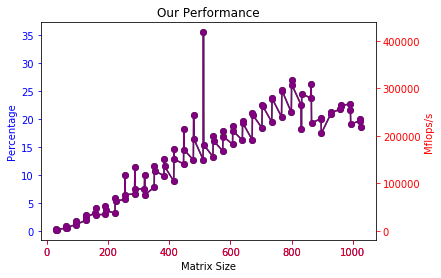
\includegraphics[width=0.6\textwidth]{blocked.png}
    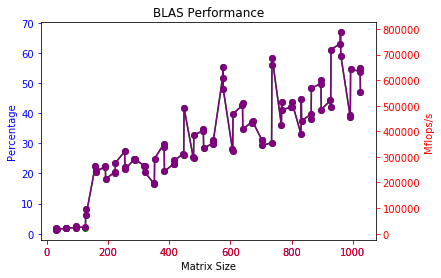
\includegraphics[width=0.6\textwidth]{blas.png}
\end{figure}



\subsection{Performance On Local Computer}
We performed the same code on a personal laptop, Lenovo Y510p with Intel i7 4700MQ 2.4 GHz, which allows AVX/AVX2 instructions. It also had the same cache specifications as Cori. The CPU allows for maximum frequency 3.4 GHz, but this was disabled. Thus this implies that the theoretical optimum is 4 cores * 2.4 GHz * 8 vector width * 2 flops for FMA = 153.6 GF/s, similar to the benchmark on Cori as well (for 4 cores). BLAS performed at 33 \%, while our blocked performed at 16 \%. This had the same behavior (i.e. outperforming Cori relatively) as part 1, possibly due to slight optimizations in Y510p's architecture. 

Note that however, the performance was much more unstable on the Y510p than on Cori, for both BLAS and blocked. Perhaps this is due to the Y510p computer's operating system not fully committing the hardware for the simulation, due to other background processes running as well. 

\begin{figure}[h]
  \caption{Performance on Lenovo Y510p, BLAS and Blocked.}
  \centering
  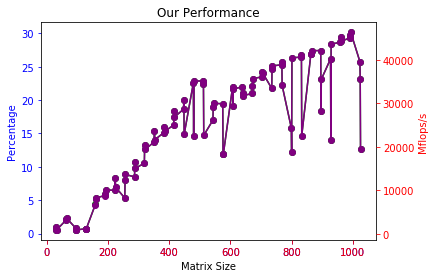
\includegraphics[width=0.6\textwidth]{blocked_local.png}
    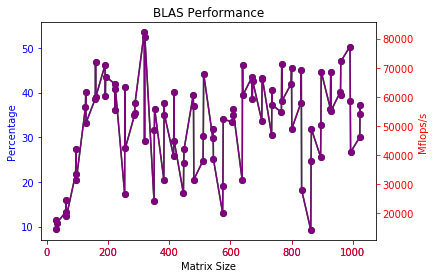
\includegraphics[width=0.6\textwidth]{blas_local.png}
\end{figure}

\newpage 
\section{Other Methods Considered}
Our other methods primarily consisted of testing where to insert the pragma omp line. As mentioned in the above method, we found that having our original parameters caused too much overhead and shared cache problems, no matter where we inserted the pragma. Furthermore, we inserted time stamps to check in our code, the primary causes of slow-down. Ultimately we found that the weird\_transformation was 20\% of the run-time for serial, while computation was 80 \%. These figures were the same after parallelization. 

% --------------------------------------------------------------
%     You don't have to mess with anything below this line.
% --------------------------------------------------------------
 
\end{document}
